\documentclass[a4paper, 11pt]{article}
\usepackage{graphicx}
\usepackage[utf8]{inputenc}    
\usepackage[french]{babel}
\usepackage[french,boxed,linesnumbered,vlined]{algorithm2e}
\usepackage{amsmath,amssymb}
\usepackage[top=4cm,bottom=4cm,left=3cm,right=3cm]{geometry}
\usepackage{dsfont}
%\usepackage{auto-pst-pdf}
\usepackage{tikz}
\usepackage{float}
\usetikzlibrary{shapes,arrows}
\graphicspath{{image/}}

\begin{document}

\makeatletter
\def\clap#1{\hbox to 0pt{\hss #1\hss}}%
\def\ligne#1{%
\hbox to \hsize{%
\vbox{\centering #1}}}%
\def\haut#1#2#3{%
\hbox to \hsize{%
\rlap{\vtop{\raggedright #1}}%
\hss
\clap{\vtop{\centering #2}}%
\hss
\llap{\vtop{\raggedleft #3}}}}%
\def\bas#1#2#3{%
\hbox to \hsize{%
\rlap{\vbox{\raggedright #1}}%
\hss
\clap{\vbox{\centering #2}}%
\hss
\llap{\vbox{\raggedleft #3}}}}%
\def\maketitle{%
\thispagestyle{empty}\vbox to \vsize{%
\haut{}{\@blurb}{}
\vfill
\vspace{1cm}
\begin{flushleft}
\usefont{OT1}{ptm}{m}{n}
\huge \@title
\end{flushleft}
\par
\hrule height 4pt
\par
\begin{flushright}
\usefont{OT1}{phv}{m}{n}
\Large \@author
\par
\end{flushright}
\vspace{1cm}
\vfill
\vfill
\bas{}{Encadrants : Emmanuel Jeannot, Corentin Travers\\Première année, filière informatique.\\\@location, le \@date}{}
}%
\cleardoublepage
}
\def\date#1{\def\@date{#1}}
\def\author#1{\def\@author{#1}}
\def\title#1{\def\@title{#1}}
\def\location#1{\def\@location{#1}}
\def\blurb#1{\def\@blurb{#1}}
\date{\today}
\author{}
\title{}
\blurb{}
\makeatother
\title{Projet programmation \emph{C} : Carcassonne}
\author{Nicolas Bouzat, Jérémie Foucault, Ismail Moumine, \\Guillaume Simon, Leo Villalba  }
\location{Bordeaux}
\blurb{%
}%

\begin{figure}[!tp]
\centering

\includegraphics[width=0.6\textwidth]{img/enseirb-matmeca}
\label{fig:logo}
\end{figure}
\maketitle
\tableofcontents

\newpage

\section*{Introduction}
   Le projet Carcassonne consiste à réaliser, en langage C, le jeu de société du même nom. Dans ce jeu, plusieurs joueurs essaient de construire des édifices (routes ou villes) à l'aide de cartes représentant des parties des dits édifices. Chaque joueur peut gagner des points en posant l'un de ses pions sur un édifice en cours de construction; le gain sera calculé en fonction de la taille de l'édifice final, si tant est que celui-ci soit complété. La contrainte principale à la pose de ces cartes est le respect des tuiles déjà placées : routes et villes ne peuvent être abruptement coupées par des champs, par exemple.\\
\indent L'objectif est de proposer une modélisation algorithmique des règles du jeu à l'aide de graphes, puis de les implémenter en langage C. L'idée est de posséder une architecture permettant de représenter visuellement le plateau de jeu, de déterminer les coups possibles à chaque tour, de calculer le score de chaque joueur ce qui permet à deux joueurs de jouer l'un contre l'autre, voire à un joueur de jouer contre une intelligence artificielle.\\
\indent Dans ce rapport, nous allons dans un premier temps définir les problèmes à résoudre pour la modélisation du jeu. Dans un second temps, nous expliciterons en détail l'architecture du programme; puis dans un troisième temps, détaillerons la réalisation et l'implémentation des algorithmes utilisés pour modéliser le jeu. Enfin, nous aborderons la réalisation de l'interface graphique, à l'aide de la bibliothèque \emph{SDL}.
    
\newpage
 
 
 \section{Définition du problème}
    \subsection{Présentation du jeu}\label{sec:presentation-jeu}
        \emph{Carcassonne} est un jeu de placement tactique dans lequel il faut construire un paysage médiéval composé de champs, routes et villes aux remparts fortifiés tels ceux de la ville éponyme. Le jeu peut se jouer jusqu'à 4 joueurs; néanmoins, seuls deux joueurs peuvent jouer, l'un contre l'autre, dans la version que nous proposons aujourd'hui.\\
	    \indent Le jeu commence avec une seule carte (ou, comme on les nommera dans le reste de ce rapport, une \textit{tuile}) posée sur le plateau, les autres étant cachées dans la pioche. Chacun son tour, les joueurs piochent une tuile et tentent de la placer, en respectant les tuiles déjà placées : les villes et les routes ne peuvent être coupées. Chaque joueur peut placer l'un de ses 10 pions, ou partisans, sur un morceau de terrain de la tuile qu'il vient de poser. Il gagnera des points lorsque le-dit terrain, qu'il soit ville ou route, sera fermé, c'est-à-dire entièrement représenté sur le plateau de jeu. Plus le terrain est grand, plus le nombre de points sera élevé. À la fin de la partie, le vainqueur sera le joueur ayant gagné le plus de points.
    
    \begin{figure}[H]
    \begin{minipage}[b]{0.50\linewidth}
      \centering 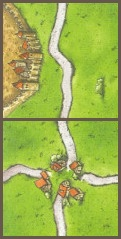
\includegraphics[scale=0.68]{img/img1.jpg}
      \caption{\it Position Permise}
   \end{minipage}\hfill
    \begin{minipage}[b]{0.50\linewidth}
      \centering 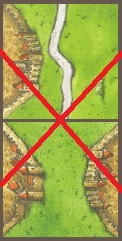
\includegraphics[scale=0.68]{img/img2.jpg}
      \caption{\it Position non Permise}
   \end{minipage}\hfill
    \label{fig:1}
    \end{figure}
    
    
    \subsection{Déroulement du jeu}
	    Chaque joueur démarre avec 10 partisans, après avoir placé sa tuile, et uniquement à ce moment-là, le joueur peut s'il le souhaite placer un pion sur une des parties de cette tuile (morceaux de villes ou de champs, tronçons de chemins, abbayes). La ville, le champ ou le chemin formé par les éléments contigus devient alors la propriété exclusive de ce joueur, et personne, pas même le propriétaire, ne pourra y placer d'autre pion en l'agrandissant par une nouvelle tuile contiguë. Cependant, une nouvelle tuile peut réunir des parties disjointes sur lesquelles il y a déjà des pions. C'est alors le joueur qui y a le plus de pions qui devient le propriétaire de l'ensemble (si les joueurs sont à égalité, le terrain appartient autant à chacun).\\
	    \indent Quand une route ou une ville est complétée, ses propriétaires comptent leurs points, et récupèrent leurs pions. Les pions placés sur les champs y restent jusqu'à la fin du jeu.\\
	    \indent Le jeu est terminé quand toutes les tuiles ont été placées. On compte alors des points pour les champs, et pour les routes et les villes non complétées.

\newpage
 
 
 
\section{Architecture du programme}

\indent L'exécution du programme \emph{Carcassonne} est détaillée figure \ref{fig:archi-prog}. Elle est régie par l'affichage et notamment par la bibliothèque \emph{SDL}. Le fonctionnement est le suivant : la librairie multimédia \emph{SDL} est tout d'abord initialisée; elle ne charge dans un premier temps que les images du menu, qu'elle affiche immédiatement. Ceci est codé dans le fichier \textsf{main.c}. Une fois que le joueur accepte de commencer une partie, le programme initialise toute la mémoire utilisé pour la gestion du plateau de jeu et des tuiles. Cette mémoire sera libérée à la fin de l'execution par appel des fonctions dédiées. Le programme charge notamment les caractéristiques de chaque tuile depuis un fichier texte \textsf{tuiles.txt}, à l'aide du parseur dont le fonctionnement est détaillé dans la section \ref{sec:autre-fct-parsing}.\\
\indent Le jeu rentre ensuite dans une boucle "infinie", définie dans \textsf{jeu.c}, au cours de laquelle \emph{SDL} attend que le joueur presse une touche, pour déplacer le curseur ou pour valider la position de celui-ci. Selon l'action, on fait alors appel aux différentes fonctions qui gèrent les graphes du plateau de jeu, dans les fichiers \textsf{plateau.c}, \textsf{graphes.c} et \textsf{regles.c}. Le résultat de ces fonctions modifie alors l'affichage, qui est rafraîchi par un appel aux fonctions du fichier \textsf{affichage.c}.





\tikzstyle{prog} = [circle, draw, fill=blue!20, 
    text width=6em, text centered, rounded corners, node distance = 4cm, minimum height = 4em]
\tikzstyle{prog2} = [circle, draw, fill=yellow!20, 
    text width=6em, text centered, rounded corners, node distance = 4cm, minimum height = 4em]
\tikzstyle{prog3} = [circle, draw, fill=green!20, 
    text width=6em, text centered, rounded corners, node distance = 4cm, minimum height = 4em]
\tikzstyle{prog4} = [rectangle, draw, fill=black!10, text width=6em, text centered, node distance = 4cm, minimum height = 4em]
\tikzstyle{line3} = [draw, <->, thick, -latex']
\tikzstyle{line} = [draw, very thick, -latex']
\tikzstyle{line2} = [draw, -latex']

    
\begin{figure}[H]
\centering
\begin{tikzpicture}[node distance = 1cm, auto]

    \node [prog](main){main.c};
    \node [prog, below of=main, node distance = 5cm](jeu){jeu.c};
    \node [prog2, left of=jeu](affichage) {affichage.c};
    \node [prog3, below right of = jeu] (plateau){plateau.c};
    \node [prog3, right of = jeu] (tuiles) {tuiles.c};
    \node [prog3, below of =jeu] (graphe) {graphes.c};
    \node [prog3, below left of = jeu] (regles) {regles.c};
    \node [prog3, right of =jeu] (graphtuile) {graphtuiles.c};
    \node [prog4, above of = tuiles] (parseur) {tuiles.txt};
    
    \path [line] (main) -- (jeu);
    \path [line3] (jeu) -- (tuiles);
    \path [line3] (tuiles) -- (jeu);
    \path [line3] (jeu) -- (plateau);
    \path [line3] (plateau) -- (jeu);
    \path [line3] (jeu) -- (graphe);
    \path [line3] (graphe) -- (jeu);
    \path [line3] (jeu) -- (regles);
    \path [line3] (regles) -- (jeu);
    \path [line] (jeu) -- (affichage);
    \path [line] (parseur) -- (tuiles);
    
\end{tikzpicture}
\caption{Architecture des fichiers du programme}
\end{figure}

\newpage

\tikzstyle{decision} = [diamond, draw, fill=red!20, 
    text width=6em, text centered, rounded corners, node distance = 4cm, minimum height = 4em]
\tikzstyle{decision2} = [diamond, dashed, fill=red!20, 
    text width=6em, text centered, rounded corners, node distance = 4cm, minimum height = 4em]
\tikzstyle{block} = [rectangle, draw, fill=green!20, 
    text width=6em, text centered, rounded corners, node distance=3cm, minimum height=4em]
\tikzstyle{fonction} = [rectangle, draw, fill=red!20, 
    text width=6em, text centered, rounded corners, node distance=3cm, minimum height=4em]
\tikzstyle{victoire} = [diamond, draw, fill=green!20, 
    text width=6em, text centered, rounded corners, node distance=4cm, minimum height=4em]
\tikzstyle{victoire2} = [diamond, dashed, fill=green!20, 
    text width=6em, text centered, rounded corners, node distance=4cm, minimum height=4em]
\tikzstyle{ia} = [rectangle, draw, fill=yellow!20, 
    text width=6em, text centered, rounded corners, node distance=3cm, minimum height=4em]



\begin{figure}[H]
\centering
\begin{tikzpicture}[node distance = 1cm, auto]
    \node [decision] (initSDL) {Initialisation de SDL };
    \node [fonction, right of=initSDL, node distance = 4cm] (menuSDL) {Affichage du Menu};
    \node [victoire, right of=menuSDL, node distance = 4cm] (initGraph) {Initialisation des graphes};
    \node [decision, right of=initGraph, node distance = 4cm] (initImg) {Chargement des images};
    \node [block, below right of=menuSDL] (pioche) {Pioche};
    \node [fonction, below left of=pioche, node distance = 4cm] (affichage1) {Affichage du jeu};
    \node [block, below of=affichage1, node distance = 4cm] (graph1) {Liaison avec graphes};
    \node [fonction, left of=graph1] (clavier1) {Touche clavier};
    \node [fonction, below right of = pioche, node distance = 4cm] (affichage2) {Affichage du jeu};
    \node [fonction, below of = affichage2, node distance = 4cm] (clavier2) {Touche clavier};
    \node [block, right of=clavier2] (graph2) {Liaison avec graphes};
    \node [block, below of= pioche, node distance = 10cm] (graph3) {Calcul du vainqueur};
    \node [fonction, below of =graph3, node distance = 2cm] (affichage3) {Affichage (fin du jeu)};
    \node [victoire2, below left of=affichage3, node distance = 3.5cm] (graph4) {Libération des graphes};
    \node [decision2, below right of=affichage3, node distance = 3.5cm] (affichage4) {Libération des images};

    
    \path [line] (initSDL) -- (menuSDL);
    \path [line] (menuSDL) -- (initGraph);
    \path [line] (initGraph) -- (initImg);
    \path [line] (initImg) |- (pioche);
    \path [line] (pioche) -- (affichage1);
    \path [line] (affichage1) -- node[left = 0.5cm]{(Pose tuile)}(clavier1);
    \path [line] (clavier1) -- (graph1);
    \path [line] (graph1) -- (affichage1);
    \path [line] (affichage2) -- (clavier2);
    \path [line] (clavier2) -- (graph2);
    \path [line] (graph2) -- node[right = 0.5cm]{(Pose partisan)}(affichage2);
    \path [line] (affichage2) -- (pioche);
    \path [line2] (graph1) -- node[sloped, very near end]{si partisans restant}(affichage2);
    \draw [draw, very thick] (pioche) -- (6.13,-5.8);
    \draw [line] (6.13, -7.3) -- (graph3);
    \draw [line] (graph3) -- (affichage3);
    \draw [line] (affichage3) -- (graph4);
    \draw [line] (affichage3) -- (affichage4);
    \draw [draw, very thick] (affichage3) -- (6.13, -19);
    \draw [draw, very thick] (6.13, -19) -- (-1.5, -19);
    \draw [draw, very thick] (-1.5, -19) -- (-1.5, -3);
    \draw [draw, very thick] (-1.5, -3) -- (4, -3);
    \draw [line] (4, -3) -- (menuSDL);
    
\end{tikzpicture}
\caption{Architecture des fonctions du programe}
\label{fig:archi-prog}
\end{figure}




\newpage

\section{Réalisation algorithmique et implémentation des fonctions logique}
 
     \subsection{Réalisation des tuiles}\label{sec:tuiles}
		\subsubsection{Réalisation algorithmique}\label{sec:tuiles-algo}
			\indent La modélisation formelle du jeu commence par l'élément principal constituant le jeu ; les tuiles. On compte parmi toute les tuiles 4 types d'éléments : 
			\begin{itemize}
				\item les champs
				\item les villes
				\item les routes
				\item les abbayes ou monastères
			\end{itemize} 
			Chacune des 24 tuiles du jeu est une combinaison unique d'un ou plusieurs de ces éléments. La première étape à donc été de choisir une modélisation adaptée pour les représenter; le modèle des graphes a été choisit. Ainsi chaque tuile est représentée par un graphe. Il s'agit d'un graphe à au plus 8 sommets, la répartition de ces sommets est donnée figure \ref{fig:sommet_disposition} et est liée à la forme carré de la carte. 
            
            \begin{figure}[H]
              \centering
    		  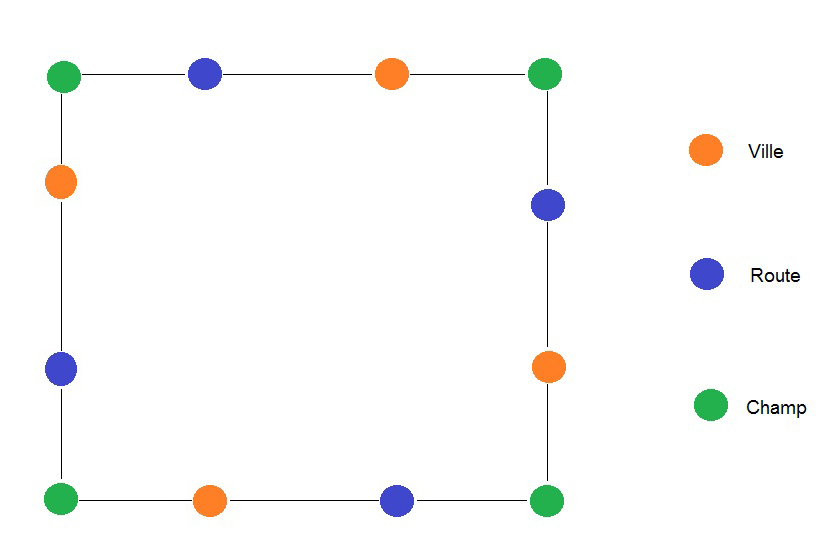
\includegraphics[width=0.7\textwidth]{img/Graphe_Tuile.jpg}
			  \caption{Sommets du graphe d'une tuile}
			  \label{fig:sommet_disposition}
			\end{figure}
            
            De plus elle est basée sur les faits suivant : 
			\paragraph{Fait 1:}il ne peut y avoir une route et une ville sur un même coté de tuile.
			\paragraph{Fait 2:}il ne peut y avoir de route sans champ.
			\paragraph{Fait 3:}il ne peut y avoir que des champs dans une tuile, au minimum une abbaye sera présente.
			\paragraph{Fait 4:}la forme triangulaire des villes implique pour notre représentation qu'un champ et une ville puisse être activé sur la même arête d'une tuile.\\

			
			\indent Partant de ces constats, le choix de n'opter que pour 4 sommets aurait pu être fait, ce qui aurait impliqué que l'absence d'information aurait signifié la présence d'un champ. Or comme nous le verrons dans la partie \ref{sec:pose-partisan-algo} des informations sur les champs nous ont semblé nécessaire pour la gestion des partisans. En résumé chaque tuile compte au plus 8 sommets qui représentent un des types d'élément constituant une tuile.  \\

			\indent Après avoir défini se que représente un sommet, nous pouvons définir le rôle d'une arête. Les arêtes ne sont pas orientées et peuvent seulement relier deux sommet de même type (route - route, ville - ville, champ - champ). Ces arêtes définissent les limites, les contours, de chaque éléments de la tuile. Ainsi par exemple deux sommets route reliés définirons une route, quand un sommet isolé représentera le début ou la fin d'une route.\\
			
			\indent Il demeure le cas particulier des abbayes, elles sont représentées par un sommet unique sans aucune arête. 

		\subsubsection{Implémentation en \emph{C}}\label{sec:tuiles-c}
			\indent Comme nous l'avons vu précédemment, les tuiles sont représentées par de petit graphe. Pour implémenter ces graphes, un tableau de sommets et une matrice de booléen est utilisé. Ils sont définis dans la structure \verb!graphe! où chacun des types de sommets est séparé ainsi on a trois tableaux de sommets : \verb!champs!, \verb!villes!, \verb!routes! qui contiennent des pointeurs vers des structures \verb!sommets! qui elles même possèdent plusieurs champs : 
			\begin{itemize}
				\item l'entier \verb!actif! qui donne le statut du sommet, car toute les tuiles n'ont pas forcement tout leur sommets activés. 
				\item l'entier \verb!pion! qui indique la présence du partisans d'un des joueurs sur ce sommet. 
				\item l'entier \verb!parcourt_graphe! qui permet la gestion du parcourt du graphe global détaillé section \ref{sec:plateau-algo}.
				\item l'entier \verb!indice_sommet! qui permet de repérer la position du sommet dans le graphe global.
				\item l'entier \verb!fin_element! qui indique si le sommet permet de fermer une ville ou une route.
				\item l'entier \verb!type! qui permet de typer le sommet en indiquant s'il s'agit d'un sommet ville, route ou champ.
			\end{itemize}
			Ce graphe est dans un structure \verb!tuile! qui contient en plus, des champs permettant la gestion de l'affichage ainsi qu'un booléen indiquant une carte spécifique avec un emblème et donc rapportant potentiellement plus de points.


	\subsection{Concrétisation du plateau de jeu}\label{sec:plateau}
		\subsubsection{Représentation algorithmique du plateau de jeu}\label{sec:plateau-algo}
			\indent D'un point de vue algorithmique le plateau de jeu est représenté par un graphe que l'on nommera \emph{graphe global}. Ce graphe est la réunion des sous-graphes constituant chaque tuiles. Il suffit d'ajouter des arêtes entre les sommets de deux tuiles compatibles et adjacent en respectant les faits suivant : 
			\paragraph{Fait 1:}l'arête ville\footnote{Une arête route, ville, champ, est une arête reliant deux sommets de type respectivement route, ville, champ} de deux tuiles différentes est prioritaire sur les arêtes champs qui sont alors interdites.
			\paragraph{Fait 2:}le nombre d'arêtes entre deux tuiles est compris entre 1 et 3.
			\paragraph{Fait 3:}Entre deux tuiles, une arête route sera accompagnée de deux arêtes champ.

			 Ainsi un plateau de jeu avec trois tuiles posée aura pour graphe celui de la figure \ref{fig:graphe-global}. La construction de se graphe se fait au fur et à mesure du jeu.  \\
		    
		    \begin{figure}[H]
		    \begin{minipage}[b]{0.45\textwidth}
		      \centering 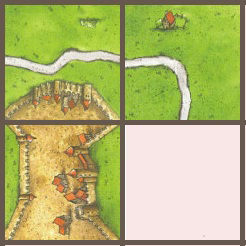
\includegraphics[width=\textwidth]{img/Trois_tuiles.jpg}
		      \caption{Exemple de 3 tuiles}
		   \end{minipage}\hfill
		    \begin{minipage}[b]{0.55\textwidth}
		      \centering 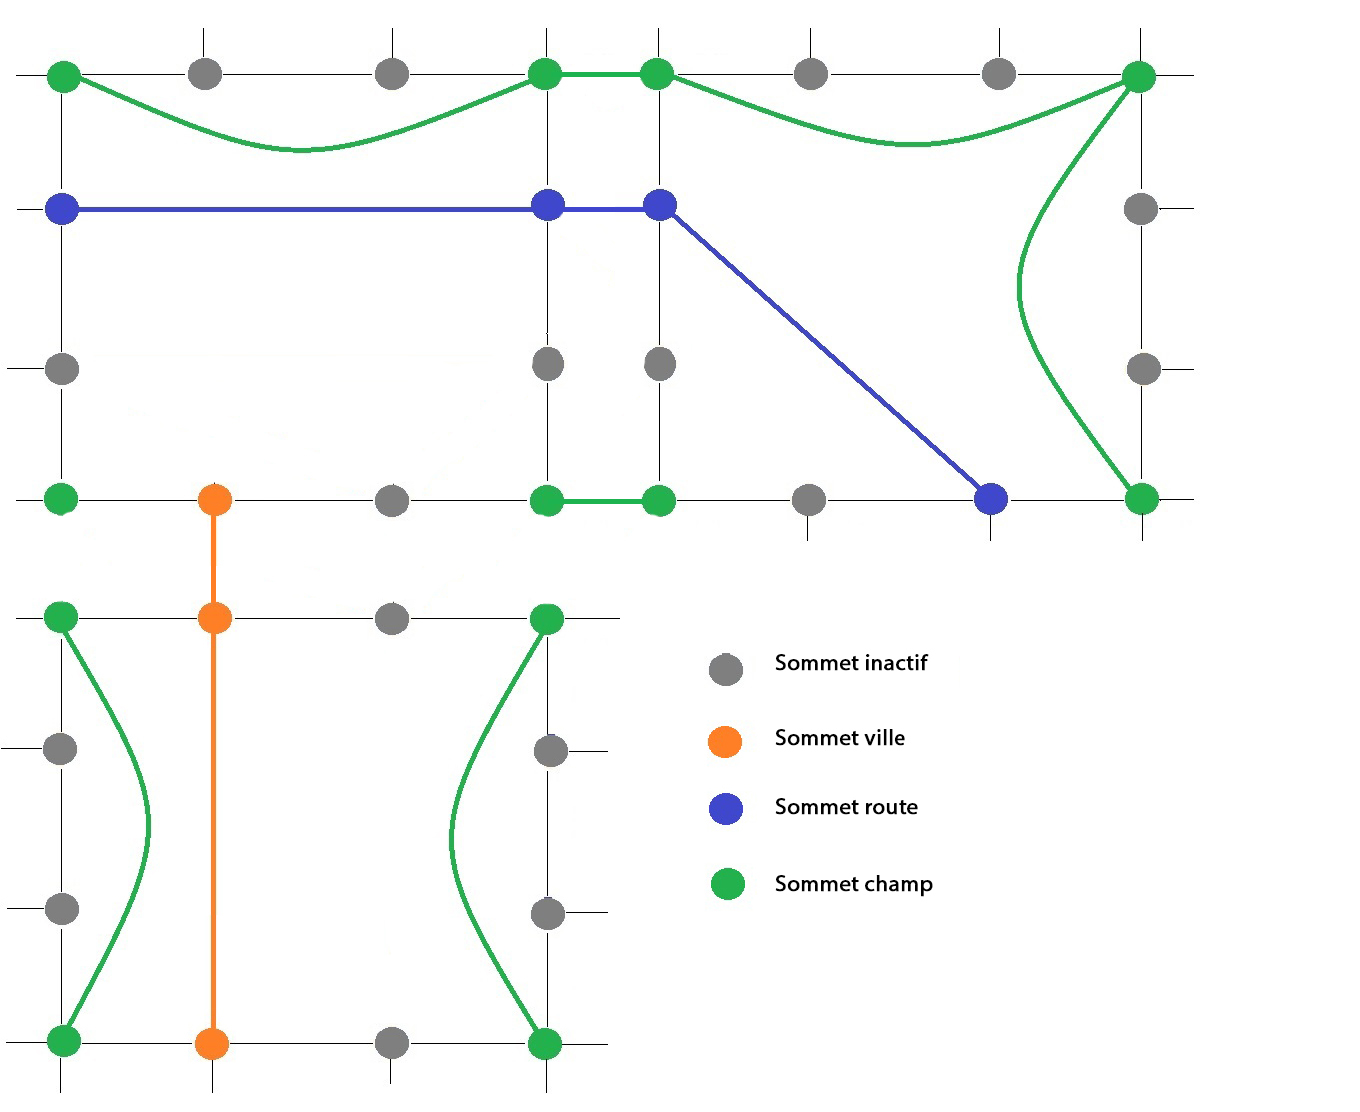
\includegraphics[width=\textwidth]{img/Graphe_trois_tuiles.jpg}
		      \caption{Graphe correspondant au 3 tuiles}
              \label{fig:graphe-global}
		   \end{minipage}\hfill
		    \end{figure}

			 \indent D'un point de vu complexité, si l'on considère que le graphe utilise une structure de type tableau de liste de successeur, l'ajout d'un sommet se fait en temps constant, l'ajout d'une arête se fait dans le pire des cas en $\Theta(m)$ où $m = |E|$. \\
			\indent Lors de l'ajout d'une tuile au graphe global, il faut donc au pire ajouter autant d'arêtes qu'il y a de sommets. Dans notre cas le nombre de sommets d'une tuile vaut 12 mais nous généraliserons ce nombre de sommet d'une tuile à la quantité $n_{sommet}$. La complexité de cet ajout est donc $\Theta(n_{sommet}\times m)$. 

		\subsubsection{Implémentation de la solution algorithmique}\label{sec:plateau-c} 
			\indent L'implémentation du plateau de jeu est réalisée de deux manières différentes mais complémentaires dans la gestion et l'application général des règles du jeu. \\
			\indent Tout d'abord le plateau est représenté par une matrice allouée dynamiquement et de taille $145\times 145$, ce qui représente le nombre maximal de tuiles que l'on pourrait aligner dans une seule direction en partant du centre. Afin d'améliorer la complexité en espace il aurait été judicieux d'utiliser une matrice à taille dynamique qui aurait été redimensionnée à chaque ajout de tuiles. Toute la mémoire allouée est évidement libérée à la fin de la partie par appel de fonctions qui y sont dédiées.
			La matrice que nous utilisons contient des pointeurs vers les tuiles qui occupent la case. Dans le cas où aucune tuile n'est placée à cet endroit, la case contient un pointeur vers \emph{NULL}. Cette matrice est particulièrement adaptée au cas de tuiles carrées et à une surface de jeu plane. Elle serait à reconsidérer dans des conditions de jeu différentes mais permet ici de gérer facilement la pose des tuiles comme il est détaillé dans la section \ref{sec:pose-tuile} \\
			\indent Néanmoins la gestion des partisans et le comptage des points doit également être réalisé. Dans cette optique le plateau est également représenté par un graphe. Ce graphe utilise un tableau de successeurs représentés par une liste chainée de structure \emph{sommet\_successeurs} contenant deux champs : 
			\begin{itemize}
				\item Un pointeur vers la structure \verb!sommets! du sommet en cours
				\item Un entier indiquant le type de l'arête entre le sommet source et le sommet en cours. Il peut s'agir d'une arrête \emph{interne} à la tuile ou \emph{externe} entre deux tuiles.
				\item Un pointeur vers le successeur suivant.
			\end{itemize}
			Ce graphe est mis à jour à chaque tour une fois qu'une tuile à été validée puis posée. Les sommets et arêtes internes à la tuile sont alors ajoutés au graphe global par réallocation de la mémoire du tableau de sommets et du tableau de successeurs. Enfin les arêtes entre cette nouvelle tuile et le graphe existant sont ajoutés. Lors de cette mise à jour du graphe les pointeurs des sommets contenus dans la tuile sont ajoutés au graphe global. Ce choix est voulu est permet ainsi de conserver une correspondance entre le plateau sous forme de matrice et celui sous forme de graphe. De plus, même si l'impact est limité, la complexité en espace est dans ce cas plus faible que la solution consistant à doubler chaque sommet. 


	\subsection{Pose des tuiles}\label{sec:pose-tuile}
		\subsubsection{Algorithme de pose}\label{sec:pose-tuile-algo}
			\indent À tours de rôle le joueur pioche une tuile qu'il doit poser sur le plateau de jeu en respectant les règles qui ont été définies dans la section \ref{sec:presentation-jeu}. Partant de se principe il est alors nécessaire de vérifier qu'une tuile posée par un joueur respecte bien les règles avant de valider la pose. Pour se faire nous utilisons l'implémentation de notre plateaux de jeux par une matrice de graphe. Ainsi il suffit de vérifier pour chacune des tuiles adjacentes aux cotés de celle qui va être posée que les sommets voisins sont compatibles comme le montre la figure \ref{fig:compatibilite-sommets}. Pour vérifier la compatibilité de deux sommets, nous avons considéré les sommets villes comme étant les plus important et donc que la seule activation de deux sommets villes sur les deux tuiles suffit à valider le coté. Viens ensuite les routes qui doivent respecter les même conditions et enfin par défaut il y aura toujours un champ. En résumé ceci revient à vérifier que deux sommets adjacents ne sont pas d'un type différent.  \\
			\indent Cette vérification s'effectue en temps linéaire en le nombre de sommets. C'est à dire dans le pire des cas, ici, $12$ sommets. On peut donc considérer que pour notre application cette vérification se fait en temps constant.

        \begin{figure}[H]
              \centering
        	  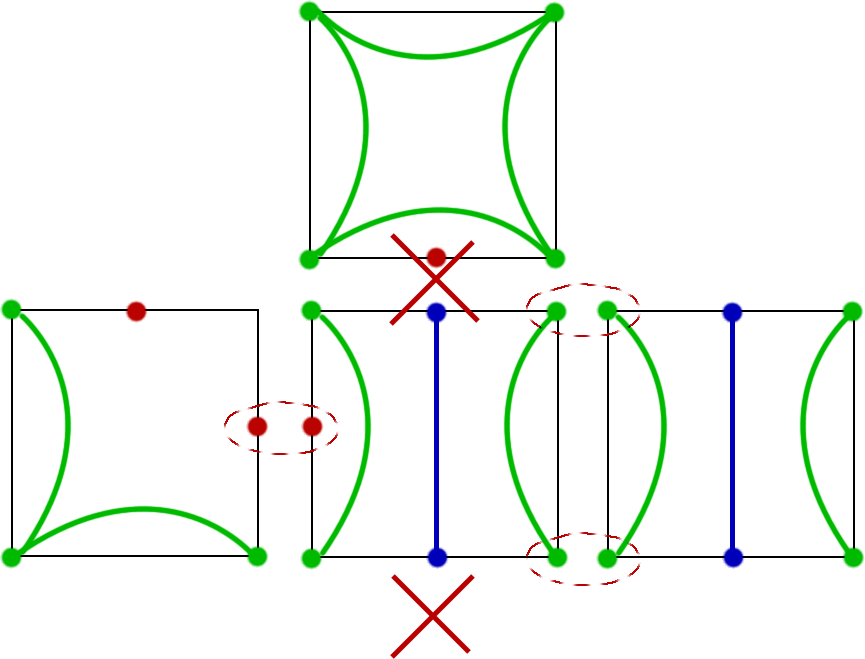
\includegraphics[width=0.7\textwidth]{img/pose-impossible.png}
			  \caption{La tuile du centre est compatible avec celles de gauche et droite, mais ne l'est pas avec celle du haut. Elle ne peut pas être posée.}
			  \label{fig:compatibilite-sommets}
		\end{figure}

		\subsubsection{Implémentation de la vérification}\label{sec:pose-tuile-c}
			\indent D'un point de vu purement algorithmique la solution détaillée précédemment est relativement simple. Cependant son implémentation s'avère plus ardue dans la mesure où de nombreux cas sont à gérer. En effet, il faut détecter la position des cartes voisines pour s'assurer de ne pas faire de tests sur le pointeur \emph{NULL}. Nous parcourons donc les quatre cases, de la matrice adjacentes, à la position de la tuiles souhaité et enregistrons les tuiles présentes. De plus afin d'améliorer la robustesse de notre programme, les cas limites sont testés, i.e, les 4 bords de notre matrice. Ensuite pour chacune des positions détectée, il suffit de vérifier que les sommets, activés, des deux tuiles correspondent. Enfin, afin de tester séparément les sommets route des sommets ville, le choix de réaliser deux fonctions a été retenu. Cependant après réalisation de l'ensemble du projet, la distinction de ces deux fonctions ne semble pas si important et une fonction générique avec un caractère indiquant le type de sommet à tester aurait probablement été plus judicieux. 


	\subsection{Pose des partisans}\label{sec:pose-partisan}
		\subsubsection{Modèle de vérification de la pose des partisans}\label{sec:pose-partisan-algo}
			\indent Les partisans constituent un rôle majeur dans ce jeu. En effet ils sont à l'origine du comptage des points et permettent donc de désigner le vainqueur d'une partie. Il est donc nécessaire de gérer la pose de ces partisans suivant les règles du jeu. Nous avons déjà rappelé que chaque joueur possède un nombre limité de partisans, 10, qu'ils doivent poser dans l'une des zone de la tuile qu'ils viennent de placer sur le plateau. \\
			\indent Dans notre jeu, la gestion des partisans et le contrôle de la pose est réalisé grâce à notre graphe représentant le plateau de jeu. Il suffit alors de parcourir tous les sommets connexes à un sommet de départ, qui correspond au sommet où l'on souhaite placer le partisans, afin de déterminer si un autre partisans occupe déjà la zone et auquel cas refuser la pose. Nous utilisons le parcourt en profondeur de l'algorithme \ref{algo:parcourt-graphe}. De plus afin d'améliorer la généricité de nos fonctions, ce parcourt générique exécutera sur chaque sommet une fonction donnée en paramètre. Ici la fonction à exécuter est \emph{est-pion} et doit retourner \emph{FAUX}. \\
			\indent Concernant la complexité, cet algorithme effectue un parcourt du graphe qui se fait en temps linéaire en le nombre de sommet et applique pour pour chacun de ces sommets une fonction qui se fait en temps constant. La complexité de cet algorithme est donc dans le pire des cas en $\Theta(m)$ où $m=|E_{graphe}|$, cependant en pratique tous les sommets ne sont pas connexe et ne sont donc pas tous parcourus.

		\begin{algorithm}[H]
		  \SetKwFunction{parcourtgraphe}{parcourt\_graphe}
		  \Entree{G:\textbf{graphe}, som:\textbf{sommet}, fct\_exec:\textbf{fonctions à exécuter}, resultat\_fct:\textbf{entier}}
		  \Sortie{Booléen}
		  \BlankLine
		  $som.couleur \leftarrow gris;$ \\
		  \Si{$\neg a\_succ(som)$}{
		  	\Retour{$Succes$}
		  }

		  \Si{$fct\_exec(som) \neq resultat\_fct$}{
		  	\Retour{$Echec$}
		  }

		  \Pour{\textbf{chaque} successeur $succ$ \textbf{de} $som$}{
		  	\Si{$est\_blanc(succ)$}{
		  		\Si{$fct\_exec(som) \neq resultat\_fct$ \textbf{ou} \\ $parcourt\_graphe(G, succ, fct\_exec, resultat\_fct) = Echec$}{
		  			\Retour{$Echec$}
		  		}
		  	}
		  }
		  $som.couleur \leftarrow noir;$ \\
		  \Retour{$Succes$}
		  \caption{Algorithme de parcourt en profondeur d'un graphe}
		  \label{algo:parcourt-graphe}
		\end{algorithm}

		


		\subsubsection{Réalisation des fonctions}\label{sec:pose-partisan-c}
			\indent La première étape est la réalisation de la fonction de parcourt du graphe, qui sera réutilisée dans la section \ref{sec:calcul-points} pour le comptage des points. Il est donc nécessaire que celle-ci soit générique. Pour se faire deux tableaux ont été utilisés : 
			\begin{itemize}
				\item un tableau de pointeur de fonctions, qui seront exécutées par ordre de rangement sur chacun des sommets lors du parcourt			
				\item un tableau d'entiers correspondant au retour de fonction attendu pour chacune des fonctions du tableau précédent.
			\end{itemize}
			L'implémentation de la fonction se fait suivant l'algorithme \ref{algo:parcourt-graphe} et le repère de sommets, déjà, ou, en cours de visite est réalisé grâce au champ \verb!parcourt_graphe! de la structure \emph{sommet}. Ce marquage des sommets parcourus implique donc une initialisation du champ de la structure pour tout les sommets avant d'effectuer un nouveau parcourt. De plus trouver l'ensemble des successeurs d'un sommet se fait par parcourt de sa liste chaînée de structures \verb!sommet_successeurs!. \\
			\indent La fonction \emph{est-pion} prend un sommet en paramètre et vérifie que ni le partisan du joueur bleu ni celui du joueur rouge n'y est posé. Cette fonction incrémente en réalité la variable \verb!nb_pions! dont le pointeur est donné en paramètre et qui correspond au nombre de pions rencontrés lors du parcourt. Cette variable est incrémenté de la façon suivante : 
			\begin{center}
				$+ 1$ pour un partisan du joueur rouge \\
				$+ 10$ pour un partisan du joueur bleu
			\end{center}
			Afin de décider si la pose d'un partisan est possible il suffit après parcourt de vérifier que la valeur de \verb!nb_pions! est nulle. On activera alors le champ \verb!pion! du sommet avec la valeur du partisan correspondant au joueur et définie par les constantes \verb!PARTISAN_BLEU! et \verb!PARTISAN_ROUGE!.

			\begin{figure}[H]
            \centering
			  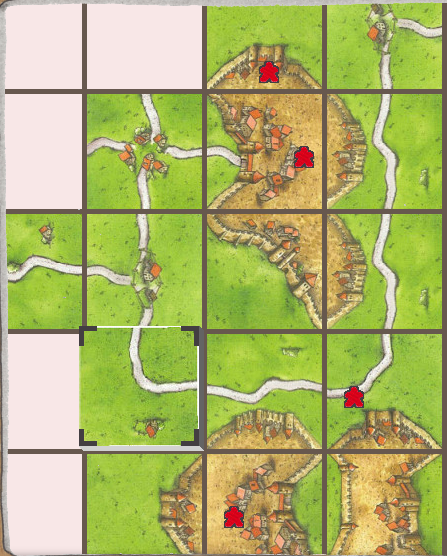
\includegraphics[width=0.7\textwidth]{img/plateau.jpg}
			  \caption{Plateau valide avec partisans}
			  \label{fig:plateau-partisans}
			\end{figure}


	\subsection{Calcul des points}\label{sec:calcul-points}
		\indent Le comptage des points se fait en deux étapes : au fur et à mesure du jeu, lorsqu'une construction de type ville ou route est terminée le nombre de points qui y est associée est calculé. Il est fonction du nombre de tuile utilisées pour la réalisation et les points sont attribuées au joueur ayant le plus de partisans sur cette construction. Dans le cas d'un nombre de partisans égal la moitié des points est attribuée à chacun des deux joueurs. Dans un second temps à la fin du jeu, les constructions de type champ sont évaluées. Des points sont attribués au joueur possédant un ou plusieurs partisans sur un champ mitoyen à une ou plusieurs villes terminées.  

		\subsubsection{Algorithme}\label{sec:calcul-points-algo}
			\indent Dans un premier temps intéressons nous au cas des constructions ville et route. Pour attribuer des points à un joueur, il est nécessaire d'effectuer un parcourt du graphe et de valider plusieurs prérequis. Nous utilisons ainsi l'algorithme de parcourt \ref{algo:parcourt-graphe} et en exécutant sur chaque sommet plusieurs fonctions. Le principe de cette fonction est donné par l'algorithme \ref{algo:calcul-points}.\\
			\indent Cet algorithme est exécuté lorsque qu'une tuile est posée sur le plateau, seulement si celle-ci est validée, sur chacun des sommets ville et route de la tuile. L'algorithme \ref{algo:calcul-points} effectue deux parcours exécutant pour chaque sommet des fonctions en temps constant. Sa complexité est donc encore une fois dans le pire des cas $\Theta(m)$ où $m=|E_{graphe}|$, mais est inférieur en moyenne. \\

			\begin{algorithm}[H]
			  \SetKwFunction{calculpoints}{calcul\_points}
			  \Entree{tuile:\textbf{graphe}, G:\textbf{graphe}, joueurs:\textbf{structure}}
			  \BlankLine
			  \Pour{\textbf{chaque} sommets (ville ou route) $som$ \textbf{de} $tuile$}{
			  	\Si{$a\_successeur(som)$}{
			  		\Si{$parcourt\_graphe(G, som, est_complet_route_ville(),Vrai)$}{
			  			\Si{$parcourt\_graphe(G, som, \{est\_pion(), marquer\_complet(),$\\$ supprimer\_pion()\},\{Vrai, Vrai, Vrai\})$}{
			  				$calcul\_score(G, som, joueurs);$
			  			}
			  		}
			  	}
			  }
			  \caption{Algorithme détectant une structure achevée et calculant le score associé}
			  \label{algo:calcul-points}
			\end{algorithm}

			\paragraph{}
			\indent Ensuite, à la fin de la partie il est possible d'évaluer les constructions champ suivant l'algorithme \ref{algo:calcul-points-champ}. Il s'agit d'un parcourt sur les sommets champ. Le principe repose sur l'exécution de l'algorithme \ref{algo:calcul-points}, en effet ce dernier marque les constructions terminées ainsi il est ici aisé de repérer un ville achevée. De plus afin de ne pas considérer deux fois une même ville lors du parcourt d'un même champ, les sommets villes achevées sont marqués comme parcourus par ce champ. \\

			\begin{algorithm}[H]
			  \SetKwFunction{calculpoints}{calcul\_points}
			  \Entree{G:\textbf{graphe}, joueurs:\textbf{structure}}
			  \BlankLine
			  \Pour{\textbf{chaque} sommets champs $som$ \textbf{de} $G$}{
			  	\Si{$est\_blanc(som)$}{
			  		\Si{$parcourt\_graphe(G, som, \{est\_pion(), est\_ville\_complete\_adjacente()\},$\\$\{Vrai, Vrai\})$}{
			  			$nb\_ville \leftarrow nb\_ville + 1;$
			  		}
			  	}
			  }
			  $calcul\_score\_champ(G, nb\_ville, joueurs);$
			  \caption{Algorithme calculant le score correspondant aux champs}
			  \label{algo:calcul-points-champ}
			\end{algorithm}

		\subsubsection{Implémentation \emph{C}}\label{sec:calcul-points-c}
			\indent L'implémentation de l'algorithme \ref{algo:calcul-points} se fait en réutilisant les idées données dans la section \ref{sec:pose-partisan-c}. Le calcul des points se fait par appel de la fonction \verb!calcul_score_pions! cette fonction détermine le nombre de partisan de chaque joueur à partir du nombre de partisans total. Cependant il faut noter que la solution choisit pourrait poser problème dans le cas ou le nombre de partisan détectés lors d'un même parcourt est supérieur à 9. Toutefois dans la mesure ou le nombre de partisans est limité à 10, il semble peu probable, mais pas improbable, que ce cas se produise. Ensuite connaissant le nombre de partisan de chaque joueurs, le nombre de tuiles et le type de structure achevée, il est possible de calculer le nombre de points et de choisir à qui les attribuer.\\

			\indent L'étape suivante de ce projet aurait été l'implémentation de la fonction d'évaluation des champ mais faute de temps cela n'a pu être réalisé. Toutefois elle aurait été implémentée en suivant l'algorithme \ref{algo:calcul-points-champ}. De plus la recherche d'une ville adjacente à un sommet champ aurait été réalisé en utilisant le fait suivant :
			\paragraph{Fait :} dans notre graphe global, si un champ est adjacent à une ville alors le sommet de cette ville a pour indice dans notre graphe \verb!sommet_indice_champ + 1!. 
			Ainsi tous les éléments nécessaire à la réalisation de cet algorithme sont réunis.


    
	\subsection{Autres fonctions et outils}\label{sec:autre-fct}
		\subsubsection{Parsing des tuiles}\label{sec:autre-fct-parsing}
			\indent Afin de charger dynamiquement et en dehors du code toutes les définitions des tuiles, un parseur à été implémenté. Les tableaux de sommets de chaque tuile sont ici définis par des séquences commençant et finissant par * sur une seule et même ligne. Ces séquences commencent par le numéro de la tuile puis sont composées de sous séquences délimitées par une lettre (c=champ, r=route, v=ville, m=monastère, e=emblème) et composées d'une suite de quatre chiffres binaires où 1 représente un sommet activé et 0 l'inverse.\\
			\indent Les matrices de booléens sont ici définies par des séquences commençant et finissant par \% sur une seule et même ligne. Ces dernières commencent par le numéro de la tuile puis sont composées de sous-séquences délimitées par une lettre (c=champ, r=route, v=ville, m=monastère) et composées d'une suite de 3 entiers le premier étant le numéro de ligne, compris entre 0 et 2, le second le numéro de colonne, compris entre 1 et 3, et le dernier la valeur du booléen (0 ou 1).\\
			\indent Les espaces ne sont pas pris en compte. Par défaut tout les sommets sont désactivés si  une séquence n'est pas renseignée, elle sera initialisée à 0000. Chaque ligne de commentaire doit commencer par \emph{\#} et se terminer par un saut de ligne. Enfin tout autre caractère que ceux mentionnées précédemment conduiront à l'échec du parsing.\\

			\indent Durant le parsing un exemplaire de chaque tuiles est alloué, et rangé dans le tableau \verb!tuiles!.


		\subsubsection{Gestion de la pioche}\label{sec:autre-fct-pioche}
			\indent La gestion de la pioche est réalisée à l'aide de la structure \verb!pioche!, allouée et libérée dynamiquement, qui contient les champs suivant : 
			\begin{itemize}
				\item \verb!tuile_pioche! qui correspond au pointeur vers la tuile piochée.
				\item \verb!nb_carte! qui est un tableau contenant le nombre de fois qu'une tuile a été piochée.
				\item \verb!nb_carte_max! qui est un tableau contenant le nombre maximal de fois qu'une tuile peut être piochée.
			\end{itemize}
			Une fonction se charge de mettre à jour la structure à chaque tours. Celle-ci, tire de manière aléatoire une tuile dans le tableau des tuiles parsées. Elle vérifie que cette tuile peut encore être tirée grâce au tableau \emph{nb\_carte\_max} et auquel cas met a jour le pointeur de \emph{tuile\_pioche} et incrémente son compteur. Sinon une autre tuile est tirée et ainsi de suite. Lors de ce tirage si la carte est disponible avant de mettre à jour le champ \emph{tuile\_pioche}, la tuile est dupliquée et c'est sa copie qui se retrouve dans la structure \emph{pioche}.


		\subsubsection{Rotation des tuiles}
		Afin de pouvoir faire tourner une tuile de 45\degre vers la gauche ou la droite, on s'est proposé d'implémenter une fonction qui applique une rotation circulaire aux sommet du graphe de la tuiles. En pratique il faut modifier les indices des tableaux de sommet et des matrices de booléens. Cette fonction modifie également le numéro de l'image associé à la tuile pour la partie graphique. Enfin précisons que cette transformation se fait par effet de bord et en temps linéaire en le nombre de sommets, on peut donc considérer ici que la rotation se fait en temps constant.


\newpage			
 
 

 

\section{Réalisation de l'interface graphique}
\indent Nous avons décidé d'utiliser la bibliothèque multimédia \emph{SDL} pour réaliser la partie graphique du jeu. Cette bibliothèque est en effet facile d'utilisation, assez puissante pour les besoins du projet et possède une importante documentation accessible sur le net. \

\subsection{Principe d'utilisation de \emph{SDL}}
\indent La bibliothèque \emph{SDL} fonctionne de la façon suivante : toute image qui doit être affichée est dans un premier temps chargée dans une variable de type SDL\_Surface. On définit ensuite des coordonnées auxquelles placer cette image, dans une variable de type SDL\_Rect. Puis on appelle la fonction SDL\_BlitSurface, qui lie image, coordonnées et surface sur laquelle afficher l'image. Ce processus est répété pour chaque image à afficher, en sachant que l'ordre d'appel de ces fonctions SDL\_BlitSurface est pris en compte; en plaçant deux images aux mêmes coordonnées, par exemple, la seconde image plaçée (dans l'ordre du code) sera superposée à la première. Une fois toutes les images placées, on appelle alors la fonction SDL\_Flip, qui affiche chacune de ces images à son emplacement dans la fenêtre \emph{SDL}. Le processus est répété à chaque appel de la fonction affichage.

\subsection{Chargement des images}
\indent Comme on vient de le voir, il est nécessaire de charger toute image à afficher dans une variable SDL\_Surface. Mais ces variables ne sont pas nécessaires au reste du programme; elles sont de fait locales à la fonction d'affichage. Afin d'éviter de devoir charger toutes les images à chaque appel de la fonction, toutes les variables SDL\_Surfaces ont été définies comme étant \textit{statiques}. Ainsi, au premier appel de "affichage", les images sont toutes chargées (à l'aide d'une condition sur un entier statique initialisé à 01 que l'on passe à 10à la fin du chargement) une seule est unique fois au cours de l'exécution du programme.\\
\indent Par souci de clarté, les images des tuiles sont chargées dans un tableau de SDL\_Surface, ce qui permettra de  les appeler facilement par le numéro de leur case. \\
\indent Enfin, par défaut, \emph{SDL} ne peut charger que des images au format bitmap (.bmp); cependant, ce format ne prend notamment pas en compte la transparence, nécessaire entre autres pour superposer des images non carrées, tels des partisans par exemple. Nous avons donc utilisé la fonction \textit{IMG\_Load} de la librairie SDL\_image.h, qui permet le chargement de fichiers de types plus divers, notamment le type Portable Network Graphics (ou PNG), qui prend en compte la transparence; c'est sous cette extension que nous avons donc enregistré toutes les images du jeu.

\subsection{Affichage du plateau de jeu}
\indent A chaque appel de la fonction d'affichage, le programme parcourt un tableau de graphes similaire à celui décrivant le plateau de jeu entier (\textit{plateau\_graphe}), nommé \textit{plateau\_visible}. Ce tableau de 4x4 cases contient les 12 tuiles que doivent être affichées à l'écran, d'après la position du curseur. La fonction lit le champ "image" de chaque tuile, qui correspond au numéro de la case du tableau de SDL\_Surface décrit précédemment; et appelle SDL\_BlitSurface pour chacune de ces images aux coordonnées voulues.
\
\subsection{Rotations de cartes}
\indent Trois solutions existaient pour traduire graphiquement la rotation de tuiles à l'écran. La première était d'utiliser la fonction \textit{rotozoom} de la bibliothèque SDL\_sfx.h, qui permet d'effectuer des rotations sur des SDL\_Surfaces définies au préalable. Cependant, afin de faciliter le travail des autres membres de l'équipe, seules des librairie \emph{SDL} installées par défaut sur les ordinateurs de l'école ont été utilisé; et SDL\_sfx.h n'en fait pas partie. Une seconde solution était d'utiliser la bibliothèque SDL\_OpenGL.h, qui est disponible à l'\emph{ENSEIRB} et qui permet d'effectuer des rotations. Cependant, \emph{OpenGL} se manipule de façon différente de \emph{SDL}, et impliquait de réécrire entièrement le code des fonctions d'affichage, ce qui nous était impossible au moment où le problème des rotations s'est posé. En outre, SDL\_OpenGL.h est beaucoup moins documentée et est extrêmement puissante comparée aux besoins de notre programme; il nous a donc semblé préférable d'abandonner cette option.\\
\indent Nous avons donc choisi la troisième option, la moins élégante mais la plus simple à implémenter dans les délais du projet. Pour chaque tuile, nous chargeons 4 images, une pour chaque orientation de la tuile. L'ordre dans lequel cette opération est effectuée est le suivant : dans les 24 premières cases (numérotées à partir de 1) du tableau de SDL\_Surfaces sont chargées les images des 24 tuiles. Dans les 24 secondes, sont chargées, dans le même ordre, 24 images de ces tuiles après une rotation de 90\degre; et ainsi de suite pour les 48 autres. Ainsi, connaissant le numéro de l'image d'une tuile que l'on veut tourner, il suffit d'ajouter ou d'enlever (selon le sens de la rotation) 24 modulo 96 à ce numéro pour obtenir celui de l'image de la tuile tournée.

\begin{figure}
\centering
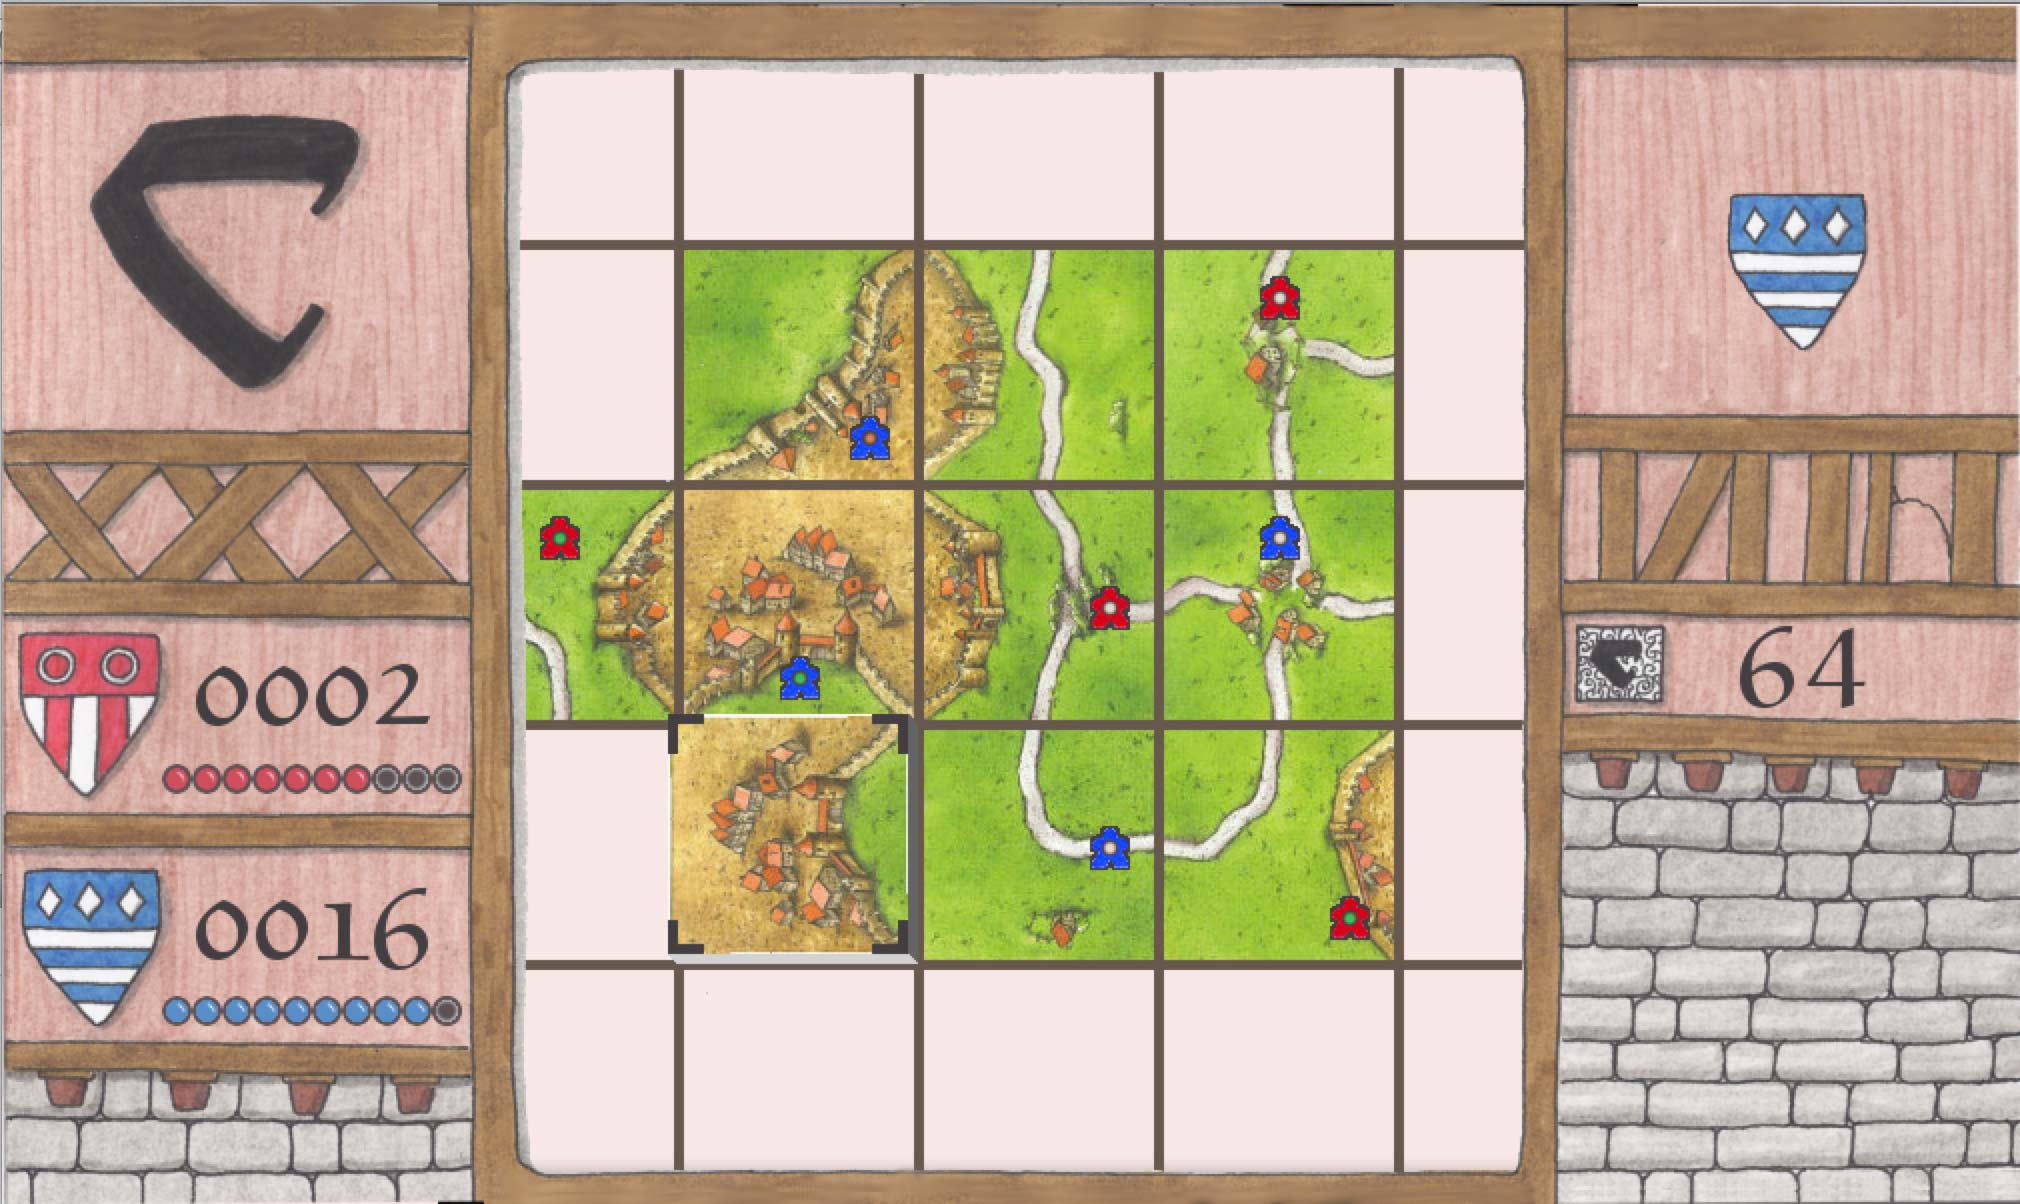
\includegraphics[width = \textwidth]{img/jeu-en-cours.png}
\end{figure}

\subsection{Compteurs de scores}
\indent Plusieurs compteurs devaient être affichés à l'écran : deux compteurs de score, ainsi qu'un compteur du nombre de cartes restantes dans la pioche et un compteur du nombre de partisans restant à chaque joueur. Si l'on a choisi d'afficher ce dernier d'une façon différente, les trois autres fonctionnent sur le même principe. \\
\indent Dans un premier temps, lors de la phase de charge des images, on charge 10 images dans un tableau de SDL\_Surface. Dans chaque case est stockée une image du chiffre correspondant au numéro de la case (la case 1 contient ainsi un chiffre "1" dans la police voulue). Dans un second temps, une fonction remplit par effet de bord un tableau d'entiers avec 4 chiffres, un par case, chaque chiffre correspondant à l'un des chiffres qui compose le score. Dans un dernier temps, il suffit alors d'appeller une boucle \emph{for} qui placera chaque image de chiffre voulue à l'endroit demandé. Le score sera ainsi mis à jour à chaque appel de la fonction affichage.c, c'est-à-dire en permanence. \\
\indent Le compteur de partisans fonctionne sur un principe plus simple; puisqu'un joueur ne peut posséder plus de 10 partisans, nous avons décidé de représenter ce compteur par 10 images, une pour chaque partisan; une boucle sur le nombre de partisans restants permet donc d'afficher à l'écran le nombre de partisans de chaque joueur.

\newpage
\section*{Conclusion}
\indent Nous avons donc réalisé, à l'issue de ce projet, un programme permettant de jouer au jeu \emph{Carcassonne}. Ce fut l'occasion de réutiliser des outils tels que \emph{Cmake} ou \emph{Doxygen} qui permettent d'améliorer l'environnement de travail, la lecture et la compréhension du code, ainsi que \emph{gdb} et \emph{Valgrind}, qui nous ont permis de corriger facilement de nombreux bugs. Ce fut de plus l'occasion de mettre en application le concept des graphes, pour un cas concret, d'un point de vu algorithmique mais également par leur implémentation. Enfin, après l'utilisation de \textit{ncurses} au premier semestre, nous avons pu découvrir une nouvelle bibliothèque graphique plus complexe.\\
\indent Nous n'avons pas pu implémenter l'ensemble des tâches requises pour ce projet : l'implémentation des abbayes n'a pas pu être réalisée, et le comptage des points obtenus par les champs n'est pas complet. En outre, nous n'avons pas eu le temps d'implémenter une intelligence artificielle. Néanmoins, notre programme final permet à deux joueurs de jouer à une version de Carcassonne relativement fidèle au jeu original. Notre modélisation des règles du jeu est fonctionnelle, et nous espérons proposer une interface graphique agréable pour l'utilisateur.

\begin{figure}[H]
\centering
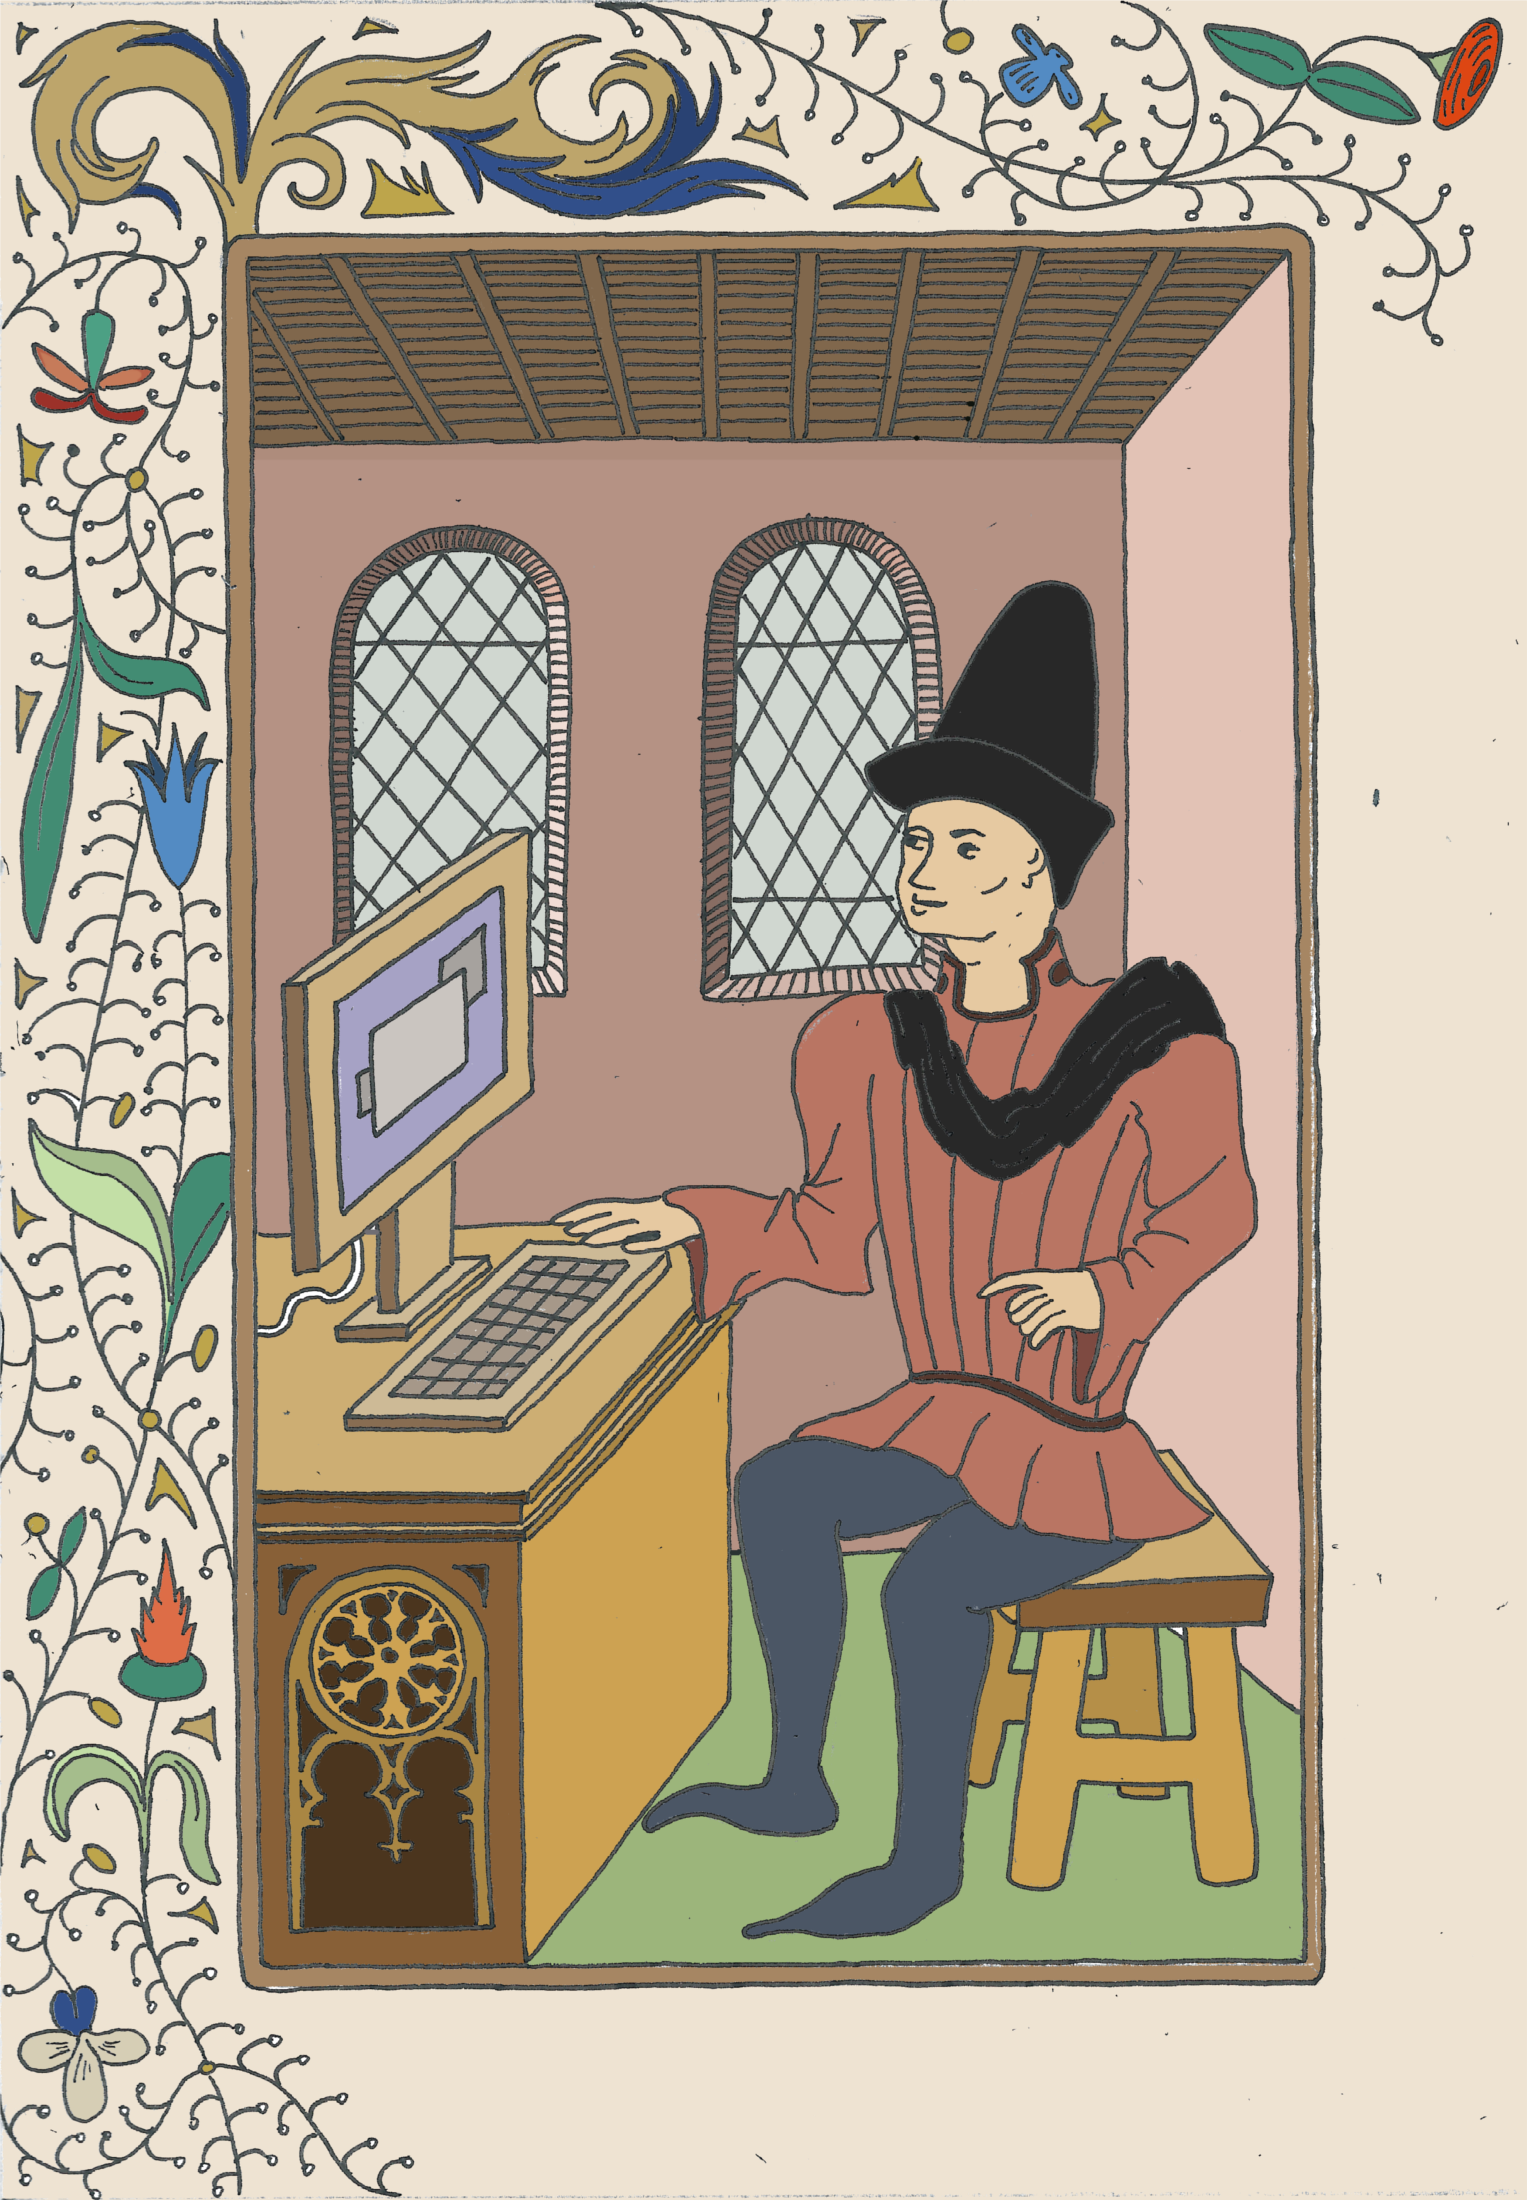
\includegraphics[width = 0.6\textwidth]{img/Enluminure_v_resized.png}
\end{figure}

\end{document}
